\documentclass[t,xcolor=pdftex,dvipsnames,table]{beamer}
\usepackage[]{graphicx}\usepackage[]{color}
%% maxwidth is the original width if it is less than linewidth
%% otherwise use linewidth (to make sure the graphics do not exceed the margin)
\makeatletter
\def\maxwidth{ %
  \ifdim\Gin@nat@width>\linewidth
    \linewidth
  \else
    \Gin@nat@width
  \fi
}
\makeatother

\definecolor{fgcolor}{rgb}{0.345, 0.345, 0.345}
\newcommand{\hlnum}[1]{\textcolor[rgb]{0.686,0.059,0.569}{#1}}%
\newcommand{\hlstr}[1]{\textcolor[rgb]{0.192,0.494,0.8}{#1}}%
\newcommand{\hlcom}[1]{\textcolor[rgb]{0.678,0.584,0.686}{\textit{#1}}}%
\newcommand{\hlopt}[1]{\textcolor[rgb]{0,0,0}{#1}}%
\newcommand{\hlstd}[1]{\textcolor[rgb]{0.345,0.345,0.345}{#1}}%
\newcommand{\hlkwa}[1]{\textcolor[rgb]{0.161,0.373,0.58}{\textbf{#1}}}%
\newcommand{\hlkwb}[1]{\textcolor[rgb]{0.69,0.353,0.396}{#1}}%
\newcommand{\hlkwc}[1]{\textcolor[rgb]{0.333,0.667,0.333}{#1}}%
\newcommand{\hlkwd}[1]{\textcolor[rgb]{0.737,0.353,0.396}{\textbf{#1}}}%
\let\hlipl\hlkwb

\usepackage{framed}
\makeatletter
\newenvironment{kframe}{%
 \def\at@end@of@kframe{}%
 \ifinner\ifhmode%
  \def\at@end@of@kframe{\end{minipage}}%
  \begin{minipage}{\columnwidth}%
 \fi\fi%
 \def\FrameCommand##1{\hskip\@totalleftmargin \hskip-\fboxsep
 \colorbox{shadecolor}{##1}\hskip-\fboxsep
     % There is no \\@totalrightmargin, so:
     \hskip-\linewidth \hskip-\@totalleftmargin \hskip\columnwidth}%
 \MakeFramed {\advance\hsize-\width
   \@totalleftmargin\z@ \linewidth\hsize
   \@setminipage}}%
 {\par\unskip\endMakeFramed%
 \at@end@of@kframe}
\makeatother

\definecolor{shadecolor}{rgb}{.97, .97, .97}
\definecolor{messagecolor}{rgb}{0, 0, 0}
\definecolor{warningcolor}{rgb}{1, 0, 1}
\definecolor{errorcolor}{rgb}{1, 0, 0}
\newenvironment{knitrout}{}{} % an empty environment to be redefined in TeX

\usepackage{alltt}
\newcommand{\SweaveOpts}[1]{}  % do not interfere with LaTeX
\newcommand{\SweaveInput}[1]{} % because they are not real TeX commands
\newcommand{\Sexpr}[1]{}       % will only be parsed by R


%\documentclass[handout,t,xcolor=pdftex,dvipsnames,table]{beamer}  % For handout
\mode<presentation>{
\useoutertheme[subsection=false]{miniframes}
%\beamertemplatenavigationsymbolsempty
\usecolortheme{custom}
\usefonttheme[onlymath]{serif}
\setbeamercovered{invisible}
%\setbeamertemplate{navigation symbols}{}
%\setbeamertemplate{mini frames}{}  % Old one
% Comment out this line to give the header
% \setbeamertemplate{headline}[default]
\setbeamertemplate{caption}[numbered]
%\setbeamertemplate{itemize items}[circle] 
\setbeamertemplate{frametitle continuation}{\frametitle{\color{white}Title}}  % So no tile on subsequent frames, from [allowframebreaks]

%%% CUSTOMISING NAVIATION %%%%
%This customises the navigation to be thin width and just have section headings (not subsections). 
\setbeamertemplate{headline}{%
\leavevmode%
  \hbox{%
    \begin{beamercolorbox}[wd=\paperwidth,ht=2.5ex,dp=1.125ex]{palette tertiary}%   % Tertiary colour is blue
    \insertsectionnavigationhorizontal{\paperwidth}{}{\hskip0pt plus1filll}
    \end{beamercolorbox}%
}}}

\RequirePackage{marvosym}

%%% INCLUDING SOLUTIONS %%%%
%% You can incorporate both questions and solutions in the 
%% same document.  Solutions can be included between the 
%% commands \begin{soln} and \end{soln}
%% To generate a pdf with only the questions uncomment:
%\excludecomment{soln}
\usepackage{comment}
\specialcomment{soln}{\begingroup \vspace{1mm} \sl}{ \leavevmode \endgroup}

%%%% DETAILS FOR PART 1 TITLE PAGE (OLD) %%%%
%\title{\large Part2 - Probability \& Distribution Theory} 
%\subtitle{} 
%\author{\copyright Dr Di Warren 2016} 
%\date{MATH1005 - Statistics}
% \colorlet{Faculty}{Arts}
%\colorlet{Faculty}{MasterBrandRed} % This is only needed if the notes are used for different faculties.
%\colorlet{FacultyText}{White}
% Defines the color of the text used on the title page and ``blocks''
% White for Business; TitlePageBlack for Arts, Pharmacy and Science
%\definecolor{CoolBlack}{rgb}{0.0, 0.18, 0.39}

%%%% DETAILS FOR FULL COURSE TITLE PAGE %%%%
\title{\Huge STATISTICS} 
\subtitle{} 
\author{\copyright University of Sydney 2017 (Di Warren)} 
\date{MATH1005}
% \colorlet{Faculty}{Arts}
\colorlet{Faculty}{MasterBrandRed} % This is only needed if the notes are used for different faculties.
\colorlet{FacultyText}{White}
% Defines the color of the text used on the title page and ``blocks''
% White for Business; TitlePageBlack for Arts, Pharmacy and Science
\definecolor{CoolBlack}{rgb}{0.0, 0.18, 0.39}

%%%% PACKAGES %%%%
\usepackage{multirow}
\usepackage{fancybox}
\usepackage[english]{babel}
\usepackage[utf8]{inputenc}
\usepackage{bm}
\usepackage{array}
\usepackage{booktabs}
\usepackage{tikz}
\usetikzlibrary{matrix,arrows,decorations.pathmorphing}
\usepackage{verbatim}
\usepackage{pgf,pgfsys,pgffor}
\usepackage{pgfplots}
\pgfplotsset{compat=1.3} %Recommended as of Pgfplots 1.3 - necessary?
\usetikzlibrary{decorations.pathreplacing,calc}
\usetikzlibrary{shapes, backgrounds}   % For Venn diagrams
\def \setA{ (0,0) circle (1cm) }
\def \setB{ (1.5,0) circle (1cm) }
\def \setC{ (0.6,1.5) circle (1cm) }
\def \setO{ (-2, -1.5) rectangle (3.5, 2.75) }
\tikzstyle{every picture}+=[remember picture]
\tikzstyle{na} = [baseline=-.5ex]
\usepackage{listings}  %Added by Di for adding R code

%\AtBeginSection[]
%{
%   \begin{frame}
 %      \frametitle{Outline}
 %      \tableofcontents[currentsection]
%   \end{frame}
%}  %This seems overkill for weekly lecture slides.

%\AtBeginSection[]
%{
%  \begin{frame}
% \frametitle{Contents}
%  \tiny{\tableofcontents[currentsection]}
%  \end{frame}
%}
%\useoutertheme{infolines} % Just lists current section in navigation at top, nice but limiting?

%%%% TITLE PAGE AND CONTENTS AT BEGINNING OF EACH TOPIC %%%%

\RequirePackage{ifthen} % package required
\newboolean{sectiontoc}
\setboolean{sectiontoc}{true} %default to true

\AtBeginSection[]
{
\begin{frame}[plain]
\vspace{60pt}
\begin{center}
\Huge{{\textcolor{MasterBrandBlue} \insertsection}}
\end{center}
\begin{tikzpicture}[scale=0.54]
%\hspace{-12pt}
%% Big Rectangle
\fill[MasterBrandRed] (0,14) -- (20,14) -- (20,15) -- (0,15);

%\draw (1,14.5) node [anchor = west] {\textcolor{MasterBrandBlue}{\Huge{\insertsection}}}; Overlays box with title, but long titles drop off the page
\end{tikzpicture} 
\end{frame}

%%%%%WORKING VERSION OF TOC%%%%%
%\begin{frame}
%   \frametitle{Outline}
%  \tableofcontents[currentsection, sectionstyle=show/hide, subsectionstyle=show/show/hide]
%  \end{frame}
%}

%%%%%2 VERSIONS - WITH AND WITHOUT TOC%%%%%
  \ifthenelse{\boolean{sectiontoc}}{
    \begin{frame}
  \frametitle{Outline}
  \tableofcontents[currentsection, sectionstyle=show/hide, subsectionstyle=show/show/hide]
 \end{frame}
  }
}
%%%%%This doesnt seem to work?%%%%
\newcommand{\toclesssection}[1]{
  \setboolean{sectiontoc}{false}
  %\section{#1}
  \setboolean{sectiontoc}{true}
}


% PDF settings
%\hypersetup{%
%  pdftitle={\inserttitle \insertsubtitle},%
%  pdfauthor={Di Warren},%
%	pdfsubject={},%
%	pdfkeywords={}%   
%	 }

%%%%  HELPFUL MACROS %%%%
\newcommand{\ud}{\mathrm{d}}
\newcommand{\var}{\mathrm{var}}
\newcommand{\ep}{\varepsilon}
\newcommand{\cov}{\mathrm{cov}}
\newcommand{\tr}{\mathrm{tr}}
\newcommand{\MSE}{\mathrm{MSE}}
\newcommand{\rank}{\mathrm{rank}}
\newcommand{\Bias}{\mathrm{Bias}}
\newcommand{\dei}{\partial}
\newcommand{\E}{\mathbb{E}}
\newcommand{\N}{\mathcal{N}}
\newcommand{\bbR}{\mathbb{R}}
\newcommand{\V}{\mathbb{V}}
\newcommand{\betahat}{\hat{\beta}}
\newcommand{\CLRM}{$\mathbf{y} = X\bm{\beta} + \bm{\ep}$}

%%%% LOGO FOR SLIDES %%%%
\logo{\vspace{79mm}
\includegraphics[height=0.9cm]{../images/sydney.pdf}}

%%%% ADD PAGE NUMBER %%%%
\setbeamertemplate{sidebar right}{}
\setbeamertemplate{footline}{%
\hfill\usebeamertemplate***{navigation symbols}
\hspace{1cm}\insertframenumber{}/\inserttotalframenumber}

%%%% BEGIN CONTENT %%%


\begin{document}



%%%% TOPIC7 %%%%
\section[7]{Topic7: Combinations of Random Variables}

\subsection[Example: Luggage Limits on A380 Flight]{Example: Luggage Limits on A380 Qantas Flight}

\begin{frame}[fragile]{Example: Luggage Limits on A380 Flight}

When booking flights, explicit luggage limits are specified, and bags are weighed at check-in. For example, for most International flights, the economy checked bag allowance is 30kg. This is essential for the safety and efficiency of the flight, as each plane has a maximum PayLoad (maximum weight allowed for passengers, crew, luggage and cargo).
\href{http://www.qantas.com/travel/airlines/checked-baggage/global/en#international-flights-excluding-north-and-south-america}{\beamergotobutton{QantasCheckedLuggageLimits}}

\begin{center}
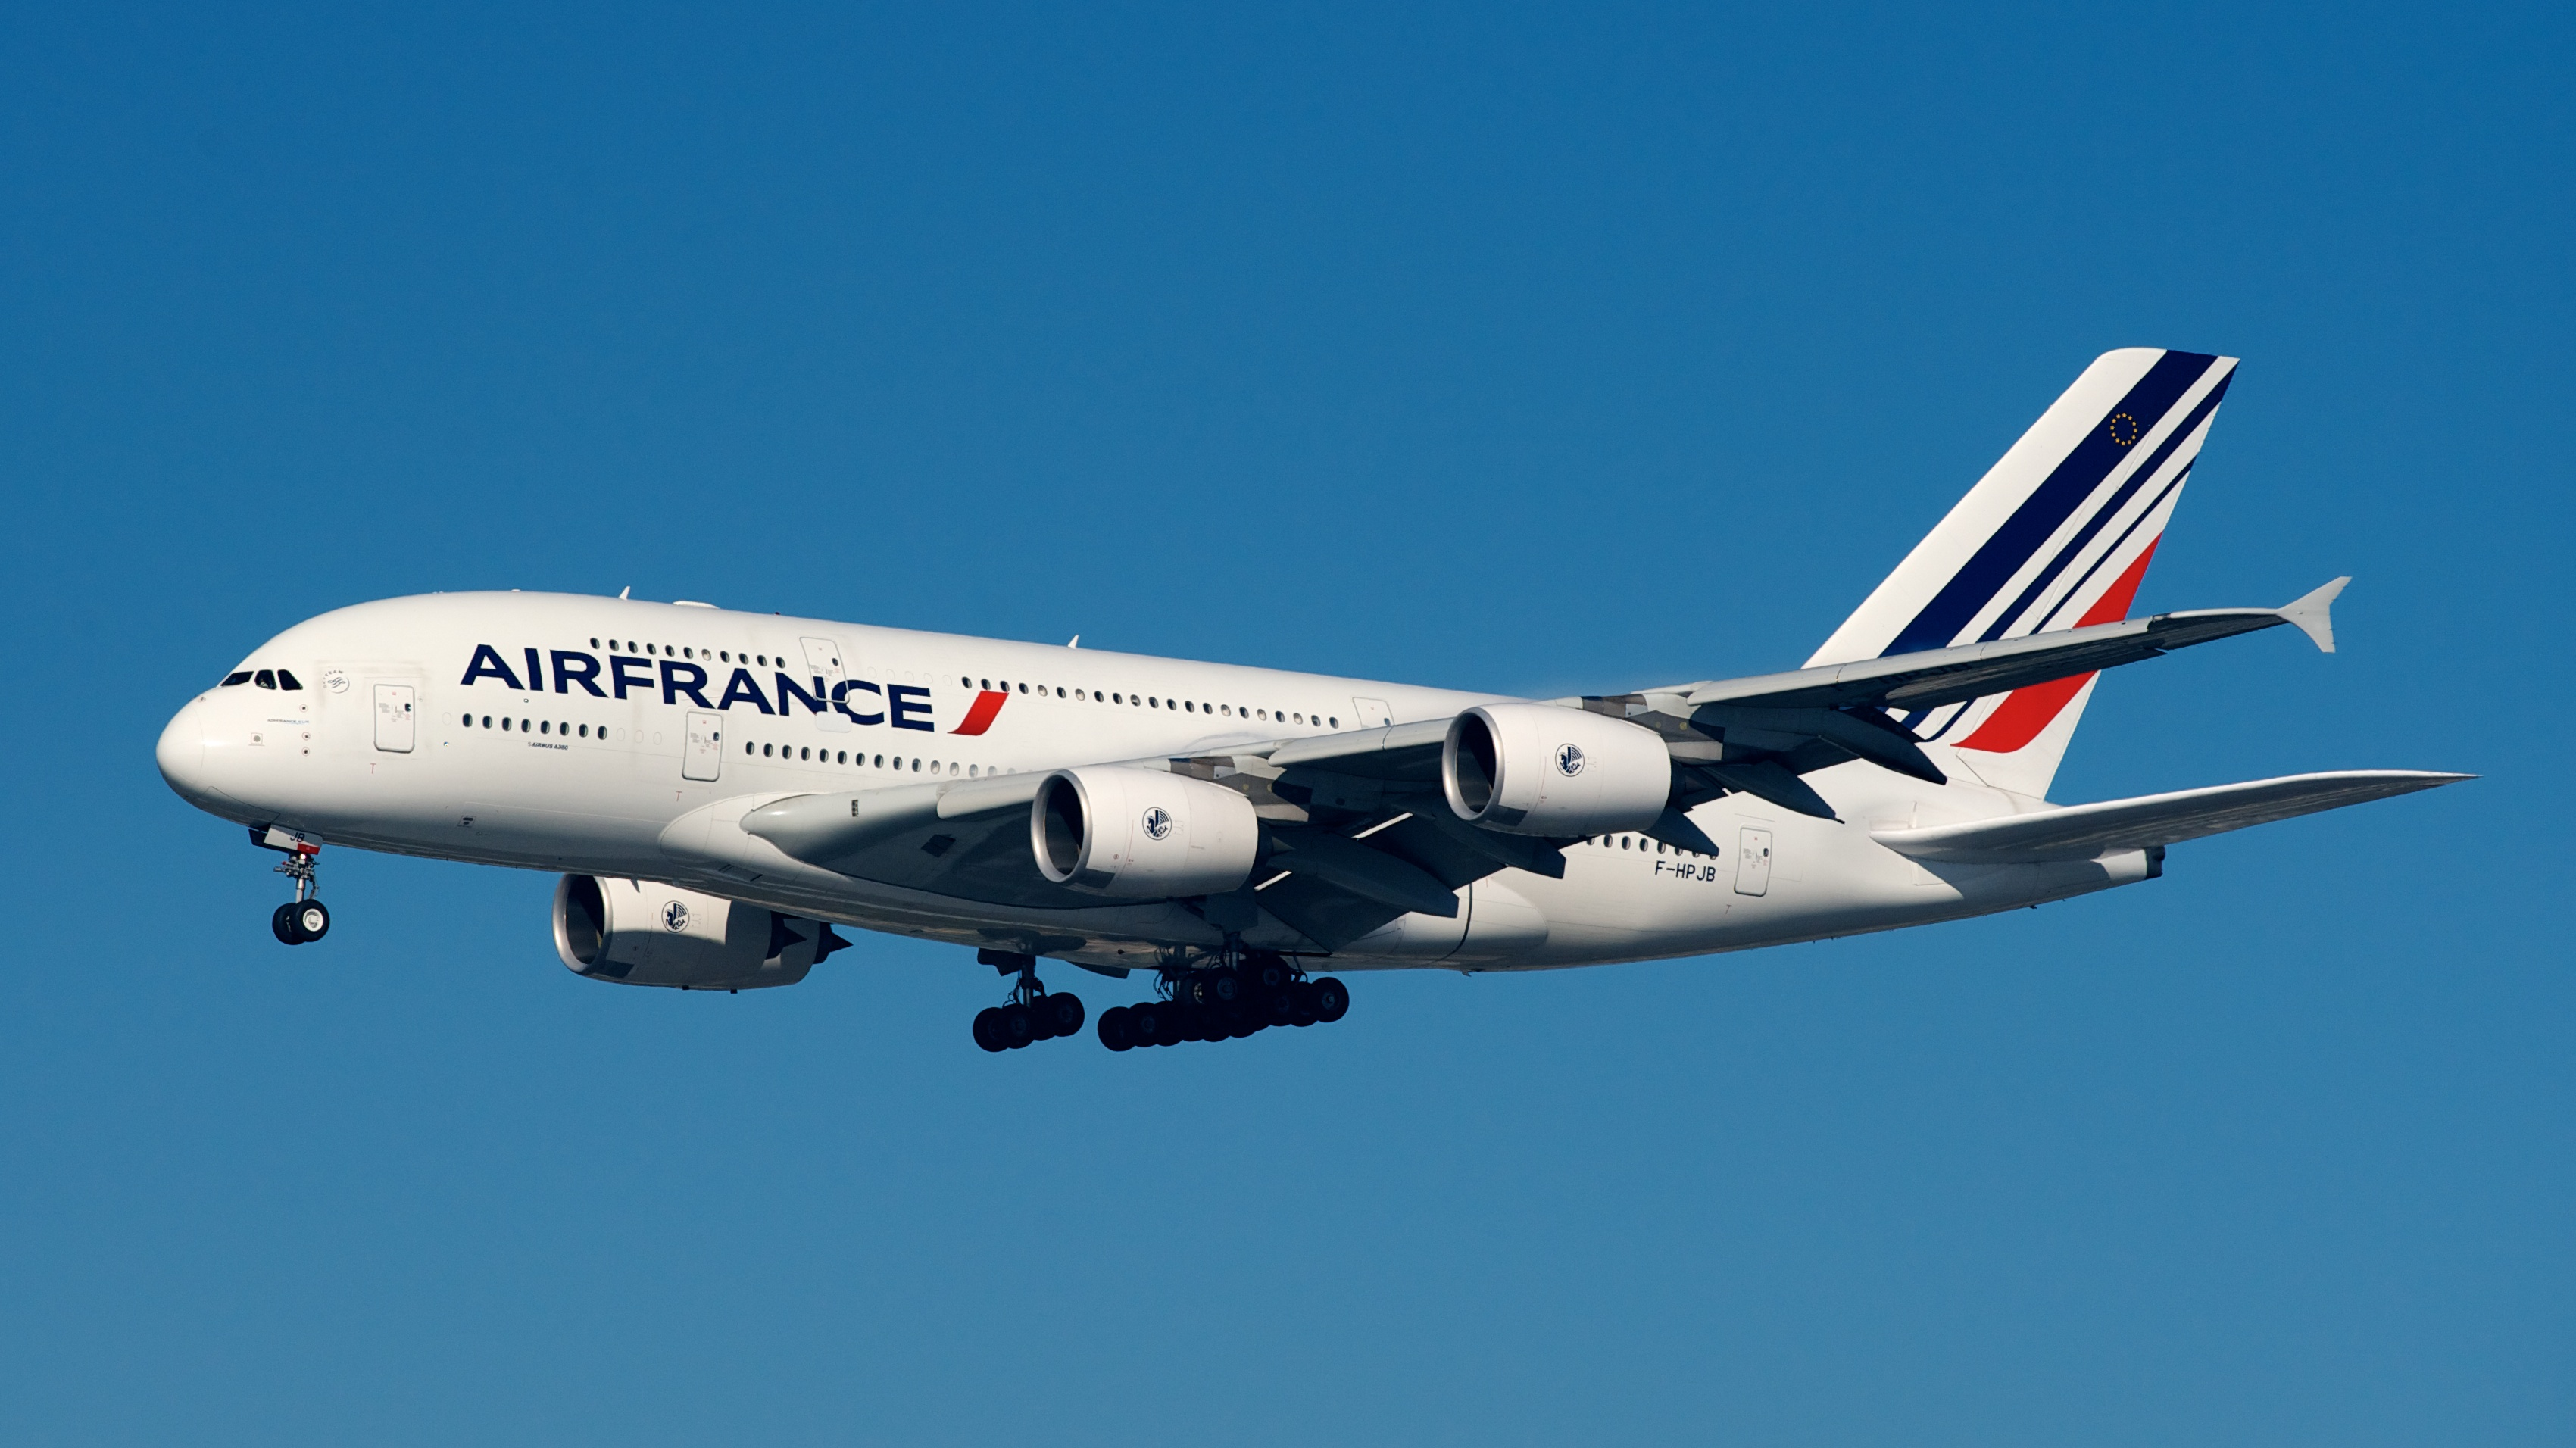
\includegraphics[height=4cm]{../images/A380.jpg}
\end{center}
\end{frame}



\begin{frame}{}

For the popular A380 plane, the Operational Weight is 270,000kg and the Zero Fuel Weight is 361,000, giving a maximum PayLoad of 91,000.
\href{hthttps://en.wikipedia.org/wiki/Airbus_A380}{\beamergotobutton{A380}}
\href{http://aviation.stackexchange.com/questions/1008/what-is-the-weight-budget-of-a-fully-loaded-a380}{\beamergotobutton{A380Specs}}

\vspace{.5cm}
{\bf What is the expected PayLoad for 530 passengers and 25 crew? Should passengers be weighed? Should hand luggage be weighted? Is it better to give a maximum luggage limit or specify limits for individual items? What baggage limits would you suggest?}

\vspace{.5cm}
Overbooking of passengers on intercontinental flights is a common practice among airlines. Aircraft which are capable of carrying 300 passengers are booked to carry 320 passengers. 

\vspace{.5cm}
{\bf If 10\% of passengers who have a booking fail
to turn up for their flights, what is the probability that at least one passenger
who has a booking, will end up without a seat on a particular flight?}

\end{frame}


\subsection[Linear Function]{Linear Function of a Random Variable}
\begin{frame}{Linear Function of a Random Variable}
\begin{definition}[Linear Function of Random Variable]
Given a random variable $X$, then $Y = a + b X$ has moments
\[ \boxed{ E(Y) = a + b E(X) } \]
and
\[ \boxed{ Var(Y) = b^2 Var(X) } \]
for all 2 constants $a$ and $b$.

\vspace{.5cm}
Special Case:
If $X \sim N(\mu, \sigma^2)$, then $Y \sim N(a + b \mu, b^2 \sigma^2)$. 

\end{definition}

Notes:  \\
(1) Expectation retains linearity. \\
(2) `A linear function of a Normal is a Normal'. This is the reason that we can standardise a Normal.
\end{frame}

\begin{frame}[fragile]\frametitle{}

\begin{block}{Example: Linear Function}
Suppose the weight of an Australian women $W \sim N(71.1, 12^2)$.
\href{http://www.abs.gov.au/ausstats/abs@.nsf/0/E11CED5FB86D178ACA257AA30014C059?opendocument}{\beamergotobutton{AustralianWeights}} \\
Find the distribution of the weight of an Australian women in pounds, given 1kg = 1 pound/2.2046.
\end{block}

\vspace{.5cm}
Let $P = \mbox{Weight of an Australian women in pounds} = 2.2406 W$. \\

This is a linear function where $a=0$ and $b= 2.2406$. \\

Hence 
\[ E(P) = 0 + 2.2406 E(W) = 2.2406 \times 71.1 =  159.3067 \]
\[ Var(P) = 2.2406^2 Var(W) = 2.2406^2 \times 12^2 = 722.9215 \]
So $P \sim N(159.3067, 26.8872^2)$
\end{frame}




\subsection[Independence]{Independence of Random Variables}

\begin{frame}{}
\begin{definition}[Independence for Random Variables]
For any random variables $X$ and $Y$, we say that \\
$X$ and $Y$ are independent
iff
\[ P(X \leq x, Y \leq y) = P(X \leq x) P(Y \leq y) \]
i.e. the joint CDF splits into the 2 individual CDFs.
\end{definition}

\vspace{.5cm}
Notes: \\
(1) 
It follows that if $X$ and $Y$ are independent, then $Cov(X,Y) = E(XY) - E(X)E(Y) = 0$. However the inverse is not true. \\
(2) You will not need to justify independence. Rather it will be assumed in any question requiring it. \\
(3) Compare to set independence:
\hyperlink{Setindependence}{\beamergotobutton{Set Independence}}
\end{frame}





\subsection[Sums]{Sums of Random Variables}

\begin{frame}{Sums of Random Variables}
\begin{definition}[Total of Random Variables]
Given any sequence of random variables $X_{1}, X_{2}, \ldots, X_{n}$, \\

the total $T = \sum_{i=1}^{n} X_{i}$ has moments
\[ \boxed{ E(T) = \sum_{i=1}^{n} E(X_{i})  } \]
and assuming independence,
\[ \boxed{ Var(T) = \sum_{i=1}^{n} Var(X_{i}) } \]

\end{definition}
\end{frame}

\begin{frame}{}
\begin{definition}[Sample Mean of Random Variables]
Given any sequence of random variables $X_{1}, X_{2}, \ldots, X_{n}$, \\

the sample mean $\bar{X} = \frac{1}{n} \sum_{i=1}^{n} X_{i}$ has moments
\[ \boxed{ E(\bar{X}) = \frac{1}{n} \sum_{i=1}^{n} E(X_{i}) } \]
and assuming independence,
\[ \boxed{ Var(\bar{X}) = \frac{1}{n^2} \sum_{i=1}^{n} Var(X_{i}) } \]
\end{definition}

These are nice results are not very useful when we don't know the shape of distribution. Hence, we will concentrate on sums of {\it Normal} random variables.
\end{frame}




\subsection[NormalSums]{Sums of Normal Random Variables}
\begin{frame}{Sums of Normal Random Variables}
\begin{definition}[Total and Sample Mean of Normal RVs]
Given a sequence of random variables $X_{i} \sim N(\mu_{i}, \sigma_{i}^2)$
(for $i=1,2\ldots,n$) \\

then  \[ \boxed{  T = \sum_{i=1}^{n} X_{i}  \sim N( \sum_{i=1}^{n} \mu_{i}, \sum_{i=1}^{n} \sigma_{i}^2    ) } \]

and
\[ \boxed{  \bar{X} = \frac{1}{n} \sum_{i=1}^{n} X_{i}  \sim N( \frac{1}{n} \sum_{i=1}^{n} \mu_{i}, \frac{1}{n^2} \sum_{i=1}^{n} \sigma_{i}^2  ) } \]

Summary: for constants $a_{i}$,
\[  \boxed{ T = \sum_{i=1}^{n}  a_{i} X_{i}  \sim N( \sum_{i=1}^{n} a_{i} \mu_{i}, \sum_{i=1}^{n} a_{i}^2
\sigma_{i}^2 ) } \]

\end{definition}
\end{frame}


\begin{frame}[fragile]\frametitle{}

\begin{block}{Example: Total}
Suppose the weight of an Australian women is $W \sim N(71.1, 12^2)$, a carry on bag is $C \sim N(6.9,0.5^2)$ and a handbag is $H \sim N(1.3, 0.4^2)$.
\href{http://www.qantas.com./travel/airlines/carry-on-baggage/global/en#carry-on-baggage-allowances}{\beamergotobutton{QantasCarryonLuggage}} \\

Find the probability that the total weight of an Australian woman with carry on luggage is more than 100kg.
\end{block}

\vspace{.5cm}
Let $T = \mbox{Total Weight of a woman with carry on luggage}$. \\

This is a sum of 3 random variables, $T = W + C + H$.

Hence 
\[ E(T) = E(W) + E(C) + E(H) = 71.1 + 6.9 + 1.3 = 79.3 \]
\[ Var(T) =  Var(W) + Var(C) + Var(H) = 12^2 + .5^2 + .4^2 = 144.41 \]
So $T \sim N(79.3, 144.41) = T \sim N(79.3, 12.01707^2)$
\end{frame}


\begin{frame}[fragile]\frametitle{}

So using standardising (Topic 6),

\[ P(T > 100) = P(\frac{T-79.3}{12.01707} > \frac{100-79.3}{12.01707}) = P(Z > 1.72255) \approx 0.04 \]

\begin{knitrout}
\definecolor{shadecolor}{rgb}{0.969, 0.969, 0.969}\color{fgcolor}\begin{kframe}
\begin{alltt}
\hlnum{1}\hlopt{-}\hlkwd{pnorm}\hlstd{(}\hlnum{100}\hlstd{,}\hlnum{79.3}\hlstd{,}\hlnum{12.01707}\hlstd{)}
\end{alltt}
\begin{verbatim}
## [1] 0.042485
\end{verbatim}
\begin{alltt}
\hlnum{1}\hlopt{-}\hlkwd{pnorm}\hlstd{(}\hlnum{1.72255}\hlstd{)}
\end{alltt}
\begin{verbatim}
## [1] 0.04248497
\end{verbatim}
\end{kframe}
\end{knitrout}
\end{frame}


\begin{frame}{}
\begin{definition}[Total and Sample Mean of iid Normal RVs]
Given a sequence of iid random variables $X_{i} \sim N(\mu, \sigma^2)$
(for $i=1,2\ldots,n$) \\

then  \[  \boxed{ T = \sum_{i=1}^{n} X_{i}  \sim N( n \mu , n \sigma^2  ) } \]

and
\[  \boxed{ \bar{X} = \frac{1}{n} \sum_{i=1}^{n} X_{i}  \sim N( \mu, \frac{\sigma^2}{n} ) } \]

\end{definition}
\end{frame}


\begin{frame}[fragile]\frametitle{}

\begin{block}{Example: Sample Mean}
Find the probability that the average weight of 10 Australian women with carry on luggage is more than 100kg.
\end{block}

\vspace{.5cm}
We have already worked out that 1 woman has a total carry on weight of $T \sim N(79.3, 12.01707^2)$. \\

\vspace{.5cm}
Now change the notation and consider a sequence of 10 women: $X_{1}, X_{2}, \ldots, X_{10}$ where $X_{i} = \mbox{carry on weight} \sim N(79.3, 12.01707^2)$. \\

\vspace{.5cm}
Assuming the women are independent, let $\bar{X} = \mbox{Average Weight of 10 women with carry on luggage}$. \\

\end{frame}


\begin{frame}[fragile]\frametitle{}

We have 
\[ \bar{X} \sim N(\mu,\frac{\sigma^2}{n}) = N(79.3, \frac{12.01707^2}{10} ) = N(79.3, 3.80013^2) \]

So using standardising,

\[ P(\bar{X} > 100) = P(\frac{\bar{X}-79.3}{3.80013} > \frac{100-79.3}{3.80013}) = P(Z > 5.447182) \approx 0 \]

\begin{knitrout}
\definecolor{shadecolor}{rgb}{0.969, 0.969, 0.969}\color{fgcolor}\begin{kframe}
\begin{alltt}
\hlnum{1}\hlopt{-}\hlkwd{pnorm}\hlstd{(}\hlnum{100}\hlstd{,}\hlnum{79.3}\hlstd{,}\hlnum{3.80013}\hlstd{)}
\end{alltt}
\begin{verbatim}
## [1] 2.558704e-08
\end{verbatim}
\begin{alltt}
\hlnum{1}\hlopt{-}\hlkwd{pnorm}\hlstd{(}\hlnum{5.447182}\hlstd{)}
\end{alltt}
\begin{verbatim}
## [1] 2.558705e-08
\end{verbatim}
\end{kframe}
\end{knitrout}
\end{frame}






\subsection[SumsNonNormal]{Sums of Non-Normal Random Variables (CLT)}
\begin{frame}{What is the Distribution of the Sample Mean for Any Population?}

If the population has distribution $X \sim ?(\mu, \sigma^2)$, what is the distribution of $\bar{X}$? We introduce a miracle theorem, which effectively allows us to use the results on Sums from the previous  section, even when the random variable are not Normal!

\vspace{.5cm}
\begin{definition}[Central Limit Theorem (CLT)]

If $X_{i} \sim  (\mu, \sigma^2)$ for $i=1,2,\ldots,n$ then

\[ \bar{X} \approx N (\mu, \frac{\sigma^2}{n}) \]

\end{definition}
\end{frame}

\begin{frame}{}

Notes:
\begin{itemize}
\item
The CLT is the most important result in this course, and in much of statistical theory.
\item
The CLT requires few assumptions:\\
\begin{itemize}
\item We must have a `big enough' sample size $n$; \\
\item
We must have finite variance $\sigma^2< \infty$.
\end{itemize}

\item 
What is a `big enough' sample size? Some textbooks give a rule of thumb (eg $n > 25$), but it all depends on the type of distribution. If $X$ is fairly symmetric, then $n$ could be small; if $X$ is highly asymmetric, then $n$ could be larger.

\item To visualise the CLT
\href{http://www.lock5stat.com/statkey/sampling_1_quant/sampling_1_quant.html}{\beamergotobutton{Lock5 Stat Key}}
\href{http://onlinestatbook.com/stat_sim/sampling_dist/}{\beamergotobutton{App}}
\end{itemize}
\end{frame}


\begin{frame}{Examples of the CLT}

(1) Uniform Distribution: $X \sim U(0,1)$, with $\mu = \frac{1}{2}$ and $\sigma^2=\frac{1}{12}$.  

\begin{knitrout}
\definecolor{shadecolor}{rgb}{0.969, 0.969, 0.969}\color{fgcolor}
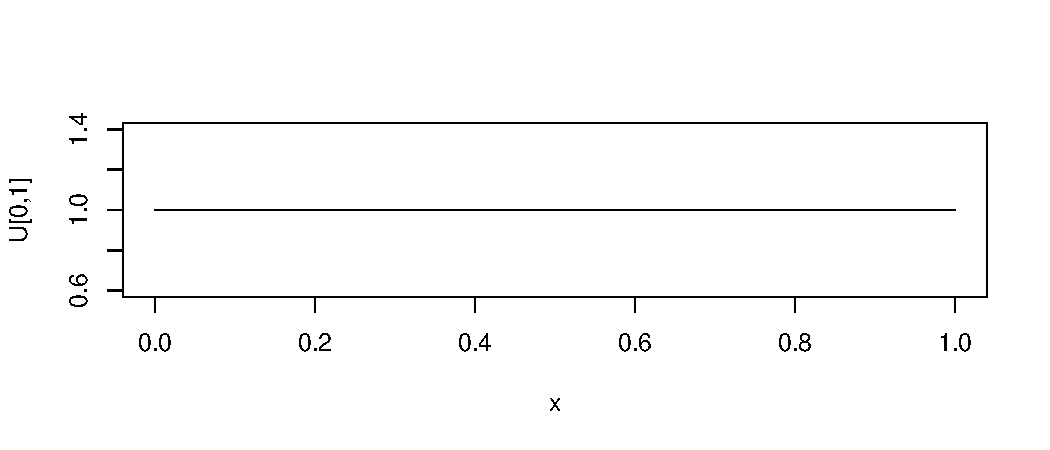
\includegraphics[width=\maxwidth]{figure/unnamed-chunk-4-1} 

\end{knitrout}

%%<<fig.height=3>>=
%%Uniform=runif(10000000,0,1)
%%hist(Uniform)
%%@

Clearly, this is a symmetric distribution.

\end{frame}


\begin{frame}{}

Simulation of Sample Mean for $n=1,2,\ldots 10$: $\bar{X} = \frac{1}{n} \sum_{i=1}^{n} X_{i}  \approx N(\mu, \frac{\sigma^2}{n}) = N(\frac{1}{2},\frac{1}{12n})$  \\


\begin{knitrout}
\definecolor{shadecolor}{rgb}{0.969, 0.969, 0.969}\color{fgcolor}
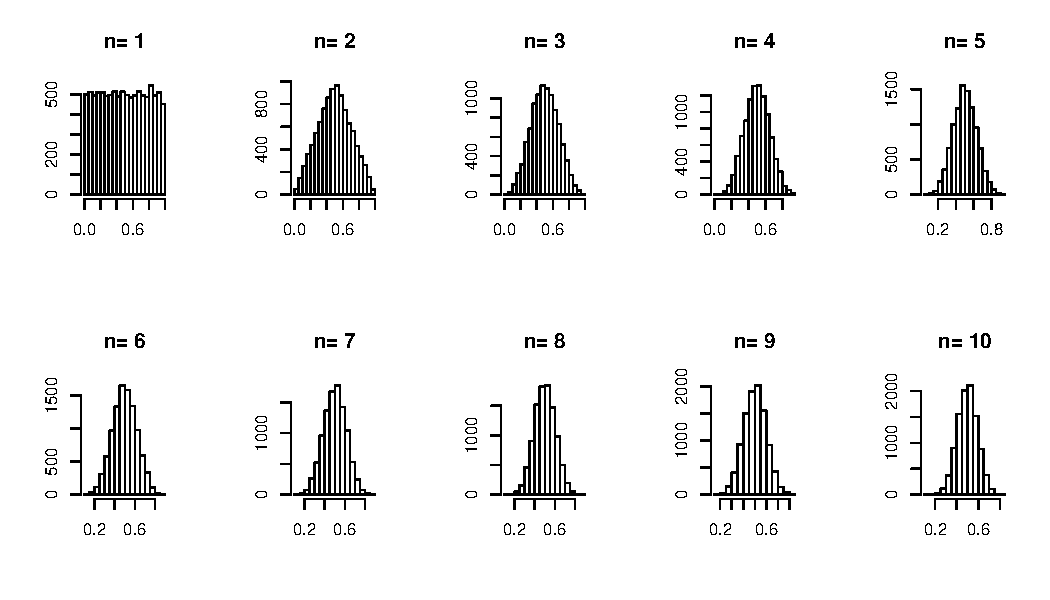
\includegraphics[width=\maxwidth]{figure/unnamed-chunk-5-1} 

\end{knitrout}
Given symmetry of $X$, $\bar{X}$ looks Normal for even $n=5$.
\end{frame}

\begin{frame}{}

(2) Binomial Distribution: $X \sim Bin(10,0.2)$, with
$\mu = 2$ and $\sigma^2 = 1.6$.

%%<<fig.height=2,echo=FALSE>>=
%%x=rbinom(10000000,10,0.2)
%%hist(x)
%%@

\begin{knitrout}
\definecolor{shadecolor}{rgb}{0.969, 0.969, 0.969}\color{fgcolor}
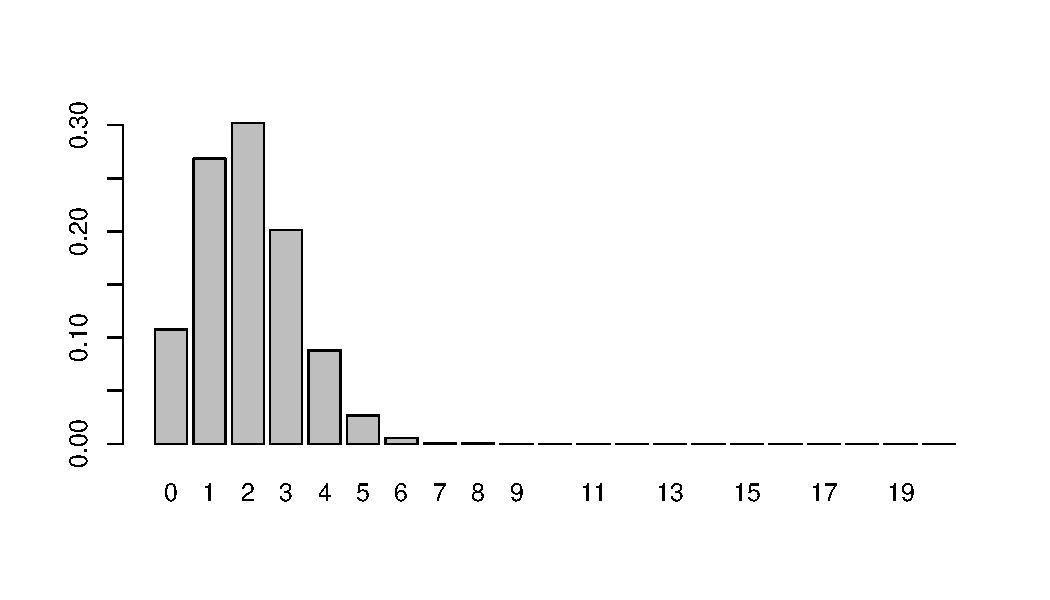
\includegraphics[width=\maxwidth]{figure/unnamed-chunk-6-1} 

\end{knitrout}

Clearly, this is a skewed distribution, as $p=0.2$.
\end{frame}


\begin{frame}{}

Simulation of Sample Mean for $n=1,2\ldots,10$: $\bar{X} = \frac{1}{n} \sum_{i=1}^{n} X_{i}  \approx N(\mu, \frac{\sigma^2}{n}) = N(2,\frac{1.6}{n})$  \\

\begin{knitrout}
\definecolor{shadecolor}{rgb}{0.969, 0.969, 0.969}\color{fgcolor}
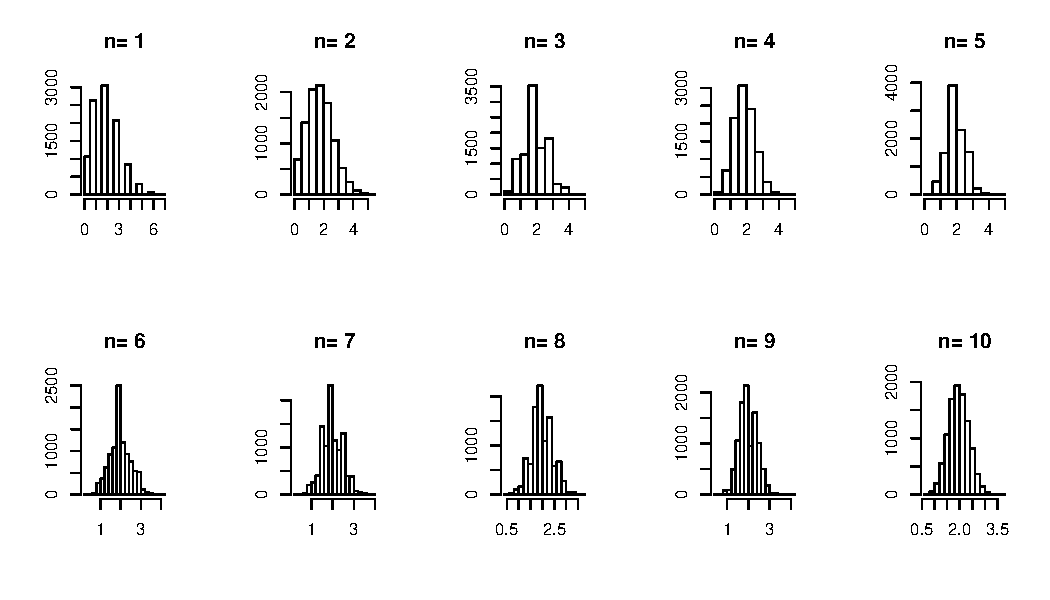
\includegraphics[width=\maxwidth]{figure/unnamed-chunk-7-1} 

\end{knitrout}

Notice, the approximation to Normal distribution, for about $n=10$.
\end{frame}



\begin{frame}{}

(3) Exponential Distribution: $X \sim Exp(0.1)$, with $\mu=10$ and $\sigma^2=100$.  \\

\begin{knitrout}
\definecolor{shadecolor}{rgb}{0.969, 0.969, 0.969}\color{fgcolor}
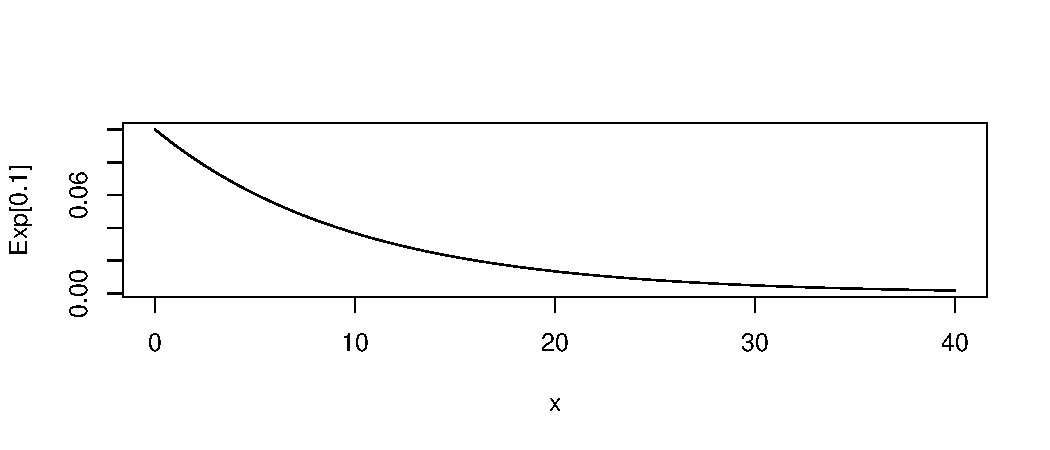
\includegraphics[width=\maxwidth]{figure/unnamed-chunk-8-1} 

\end{knitrout}

This is a highly skewed distribution.
\end{frame}

\begin{frame}{}

Simulation of Sample Mean for $n=50$: $\bar{X} = \frac{1}{n} \sum_{i=1}^{n} X_{i}  \approx N(\mu, \frac{\sigma^2}{n}) = N(10,\frac{100}{n})$  \\

\begin{knitrout}
\definecolor{shadecolor}{rgb}{0.969, 0.969, 0.969}\color{fgcolor}
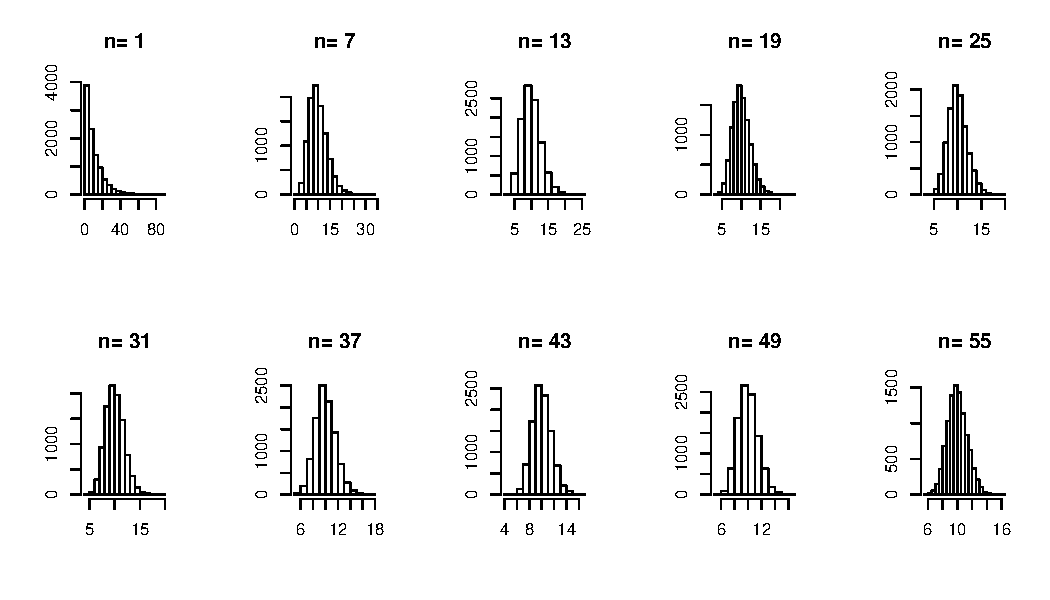
\includegraphics[width=\maxwidth]{figure/unnamed-chunk-9-1} 

\end{knitrout}

Notice, the approximation to Normal distribution, for $n=50+$.
\end{frame}

\begin{frame}[fragile]{}

\begin{block}{Example: CLT}

Assume that checked in luggage is highly skewed, as most people pack to the limit of 32kg, so $L \sim (31.9, 1^2)$.
Find the probability that the average weight of the checked in luggage of 555 passengers and crew (independent) is over 32 kg.
\end{block}

\vspace{.5cm}
Consider the 555 bags: $L_{1}, L_{2}, \ldots, L_{555}$ where $L_{i} = \mbox{checked in luggage} \sim (31.9, 1^2)$.

\vspace{.5cm}
Assuming independence, let $\bar{L} = \mbox{Average Weight of the checked in luggage}$.

\vspace{.5cm}
Using the CLT,
\[ \bar{L} \approx  N(\mu,\frac{\sigma^2}{n}) = N(31.9, \frac{1^2}{555} ) = N(31.9, 0.04244764^2) \]

\end{frame}


\begin{frame}[fragile]{}
So using standardising,

\[ P(\bar{L} > 32) = P(\frac{\bar{L}-31.9}{0.04244764} > \frac{32-31.9}{0.04244764}) = P(Z > 2.355844) \approx 0 \]

\begin{knitrout}
\definecolor{shadecolor}{rgb}{0.969, 0.969, 0.969}\color{fgcolor}\begin{kframe}
\begin{alltt}
\hlnum{1}\hlopt{-}\hlkwd{pnorm}\hlstd{(}\hlnum{32}\hlstd{,}\hlnum{31.9}\hlstd{,}\hlnum{0.04244764}\hlstd{)}
\end{alltt}
\begin{verbatim}
## [1] 0.009240349
\end{verbatim}
\begin{alltt}
\hlnum{1}\hlopt{-}\hlkwd{pnorm}\hlstd{(}\hlnum{2.355844}\hlstd{)}
\end{alltt}
\begin{verbatim}
## [1] 0.009240338
\end{verbatim}
\end{kframe}
\end{knitrout}
\end{frame}



\subsection[CLTBinomial]{Application of the CLT to the Binomial Distribution}

\begin{frame}{Application of the CLT to the Binomial Distribution}

\begin{definition}[CLT for Binomial]

For the exact Binomial $X \sim  Bin(n,p)$, the approximating Normal is
$ Y \approx N (np, np(1-p))$.

\vspace{.5cm}
Given we are approximating a discrete distribution by a continuous distribution, we usually improve the approximation by using a continuity correction (cc).
\end{definition}

\end{frame}

\begin{frame}[fragile]{}
If $X \sim Bin(10,0.6)$, and we want $P(X \leq 6)$, then we would find the Normal approximation from 6.5.

\begin{knitrout}
\definecolor{shadecolor}{rgb}{0.969, 0.969, 0.969}\color{fgcolor}
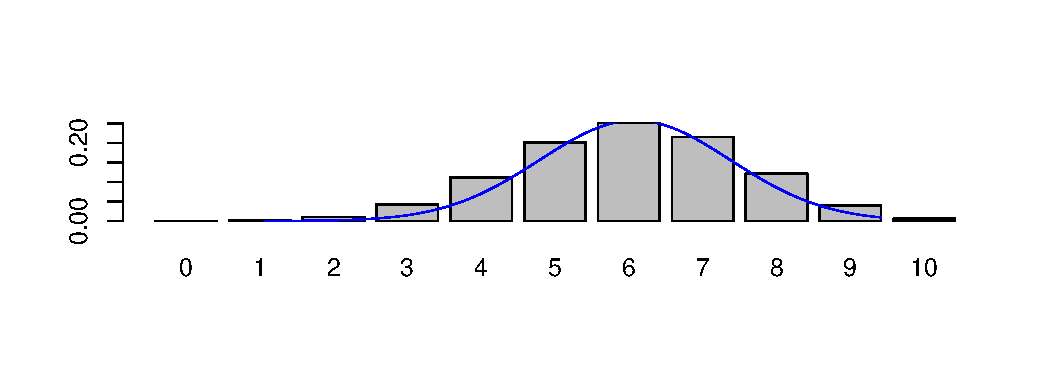
\includegraphics[width=\maxwidth]{figure/unnamed-chunk-11-1} 

\end{knitrout}

{\tiny 
\begin{knitrout}
\definecolor{shadecolor}{rgb}{0.969, 0.969, 0.969}\color{fgcolor}\begin{kframe}
\begin{alltt}
\hlkwd{pbinom}\hlstd{(}\hlnum{6}\hlstd{,}\hlnum{10}\hlstd{,}\hlnum{0.6}\hlstd{)}
\end{alltt}
\begin{verbatim}
## [1] 0.6177194
\end{verbatim}
\begin{alltt}
\hlkwd{pnorm}\hlstd{(}\hlnum{6.5}\hlstd{,}\hlnum{10}\hlopt{*}\hlnum{0.6}\hlstd{,}\hlnum{10}\hlopt{*}\hlnum{0.6}\hlopt{*}\hlnum{0.4}\hlstd{)} \hlcom{# With cc}
\end{alltt}
\begin{verbatim}
## [1] 0.5825156
\end{verbatim}
\begin{alltt}
\hlkwd{pnorm}\hlstd{(}\hlnum{6}\hlstd{,}\hlnum{10}\hlopt{*}\hlnum{0.6}\hlstd{,}\hlnum{10}\hlopt{*}\hlnum{0.6}\hlopt{*}\hlnum{0.4}\hlstd{)}  \hlcom{# Without cc}
\end{alltt}
\begin{verbatim}
## [1] 0.5
\end{verbatim}
\end{kframe}
\end{knitrout}
}
\end{frame}

\begin{frame}[fragile]{}

\begin{block}{Example: CLT for Binomial}
Assume that 90\% of passengers pack over the checked in limit of 32kg. In a random sample of 30 passengers, what is the probability more than 28 have overpacked.
\end{block}

\vspace{.5cm}
{\bf Exact Solution:} \\
Let $X = \mbox{number of passengers that have overpacked} \sim Bin(n=30,p=0.9)$. \\

\[ P(X \geq 29) = 0.183695 \]

{\tiny 
\begin{knitrout}
\definecolor{shadecolor}{rgb}{0.969, 0.969, 0.969}\color{fgcolor}\begin{kframe}
\begin{alltt}
\hlkwd{dbinom}\hlstd{(}\hlnum{29}\hlstd{,}\hlnum{30}\hlstd{,}\hlnum{0.9}\hlstd{)} \hlopt{+} \hlkwd{dbinom}\hlstd{(}\hlnum{30}\hlstd{,}\hlnum{30}\hlstd{,}\hlnum{0.9}\hlstd{)}
\end{alltt}
\begin{verbatim}
## [1] 0.183695
\end{verbatim}
\begin{alltt}
\hlnum{1}\hlopt{-}\hlkwd{pbinom}\hlstd{(}\hlnum{28}\hlstd{,}\hlnum{30}\hlstd{,}\hlnum{0.9}\hlstd{)}
\end{alltt}
\begin{verbatim}
## [1] 0.183695
\end{verbatim}
\end{kframe}
\end{knitrout}
}
\end{frame}

\begin{frame}[fragile]{}

{\bf Approximation:} \\
Exact Binomial: $X \sim Bin(n=30,p=0.9)$ \\
Approximating Normal (CLT): $Y \sim N(np,np(1-p)) = N(27,2.7) = N(27,1.643168^2)$

\vspace{.5cm}
So first using a continuity correction (cc),
\[ P( X \geq 29) \approx P(Y \geq 28.5) \]

and then standardising,

\[ P(Y \geq 28.5) = P(\frac{\bar{Y}-27}{1.643168} \geq \frac{28.5-27}{1.643168}) = P(Z \geq 0.9128707) \approx 0.18 \]

{\tiny 
\begin{knitrout}
\definecolor{shadecolor}{rgb}{0.969, 0.969, 0.969}\color{fgcolor}\begin{kframe}
\begin{alltt}
\hlnum{1}\hlopt{-}\hlkwd{pnorm}\hlstd{(}\hlnum{28.5}\hlstd{,}\hlnum{27}\hlstd{,}\hlnum{1.643168}\hlstd{)}
\end{alltt}
\begin{verbatim}
## [1] 0.1806553
\end{verbatim}
\begin{alltt}
\hlnum{1}\hlopt{-}\hlkwd{pnorm}\hlstd{(}\hlnum{0.9128707}\hlstd{)}
\end{alltt}
\begin{verbatim}
## [1] 0.1806553
\end{verbatim}
\end{kframe}
\end{knitrout}
}

\end{frame}

\end{document}
